%************************************************
\chapter{The Dean Stark Apparatus}
%************************************************
\begin{flushright}
March 11, 2013
\end{flushright}
\section{Aim}
To use the Dean Stark apparatus for separating water from a less dense reaction mixture.

\section {Chemicals Required}
	% \begin{figure}[bth]
	% 	\begin{center}
	% 		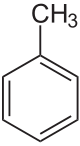
\includegraphics[width=0.1\linewidth]{gfx/e7_compound}
	% 	\end{center}
	% \caption[Aniline]{\label{e7_compound}}
	% \end{figure}


	\begin{enumerate}
		\item Water
		\item Toluene, refer to \autoref{e7_compound}
	\end{enumerate}


	\begin{figure}[bth]
		\begin{center}
			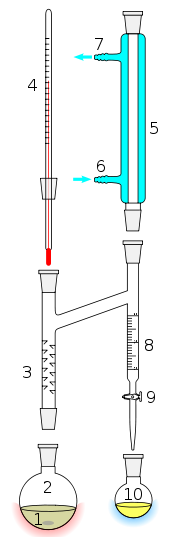
\includegraphics[width=0.4\linewidth]{gfx/e8_setup}
		\end{center}
	\caption[2-Naphthol]{\label{e8_setup}}
	\end{figure}
\section {Apparatus/Setup}
	The setup of this experiment has been given in \autoref{e8_setup} (from wikipedia). The details are as follows:
	\begin{enumerate}
		\item Heating Beads
		\item Reactants' RBF
		\item Thermometer
		\item Condenser
		\item Cooling water in
		\item Cooling water out
		\item Burette
		\item Tap
		\item Collection RBF
	\end{enumerate}

\section{Theory}
	This is by far amongst the most simplistic and elegant solutions to a seemingly deal-breaking problem. So consider any reaction which is reversible and takes place at a high temperature. Also assume that at this temperature, the reactant mixture is azeotropic with a reactant and a by-product, but they're otherwise insoluble. Further assume that the reactant is less dense than the by-product. So our objective is to separate the reactant and the by-product to ensure the reaction proceeds in the desired direction.
	\par
	Ordinary techniques fail for achieving this. Dean-stark comes to the rescue here. The setup has already been shown. The reaction mixture is boiled and its vapours travel up. Now here's the trick. When they condense after the fractional distillation setup, they get collected in the burette which is connected to the reaction mixture as shown. After condensing, the components of the mixture separate out (as they're not miscible at room temperature). The heavier of the two components, viz. the by-product settles at the bottom. The reactant goes back into the reaction mixture to continue the forward reaction. If the by-product accumulates, it can be removed easily, using the tap.

\section{Procedure}
	\begin{enumerate}
		\item The reaction mixture was emulated by using a Toluene and water mixture in the reactants' RBF (the boiling chips were added at this stage itself)
		\item The system was setup as shown in \autoref{e8_setup}. The glassware was thermally isolated using cotton and aluminium to avoid unnecessary cooling.
		\item Toluene was added to the burette at a level where it just starts to flow into the reaction mixture.
		\item The water circulator was turned on after submersing it in a large water bath.
		\item The heating was initiated and temperature monitored to keep it in the 100-110 $^o C$ range
		\item The liquid took some time, but eventually started coming out in the collection flask, while the temperature was maintained constant.
		\item The process was halted after a suitable amount of time and allowed to cool.
	\end{enumerate}

\section{Observations and Results}
	The stable thermometer read out for the boiling mixture of Toluene and water was approximately $104 ^o C$. Water was successfully removed from the `reactant mixture'. 

\section{Precaution}
	\begin{enumerate}
		\item The setup was ensured to be properly insulated, else the procedure takes too long owing to excessive cooling.
	\end{enumerate}
	Precautions given for the previous experiment must be taken here too.
	\begin{enumerate}
		\item The temperature of the thermometer would drop once one component has been separated. This doesn't mean the liquid is at that temperature, just that there isn't enough vapour in contact with the thermometer.
		\item Clean the thermometer holder in the apparatus, else there would be latency in reflection of temperature on the meter.	
		\item Do not forget to use boiling chips, else unequal heat spread may result in explosive circumstances
		\item The water output should be facing upwards
		\item The condenser tube should be sufficiently slanted in the right direction to ensure the condensed liquid flows to the receiving flask and not the other way.
	\end{enumerate}

	
\section{Acknowledgements}
I thank Dr. R Vijaya Anand for his guidance during the experiment. I also acknowledge the contribution of my lab partners, Srijit, Prashansa, Vivek, Saumya, Manisha and Sandhya for performance of the same. I also thank our PhD guide for demonstrating the experiment and her assistance in general, with performance of the same.

	% \clearpage
	% \begin{figure}[bth]
	% 	\begin{center}
	% 		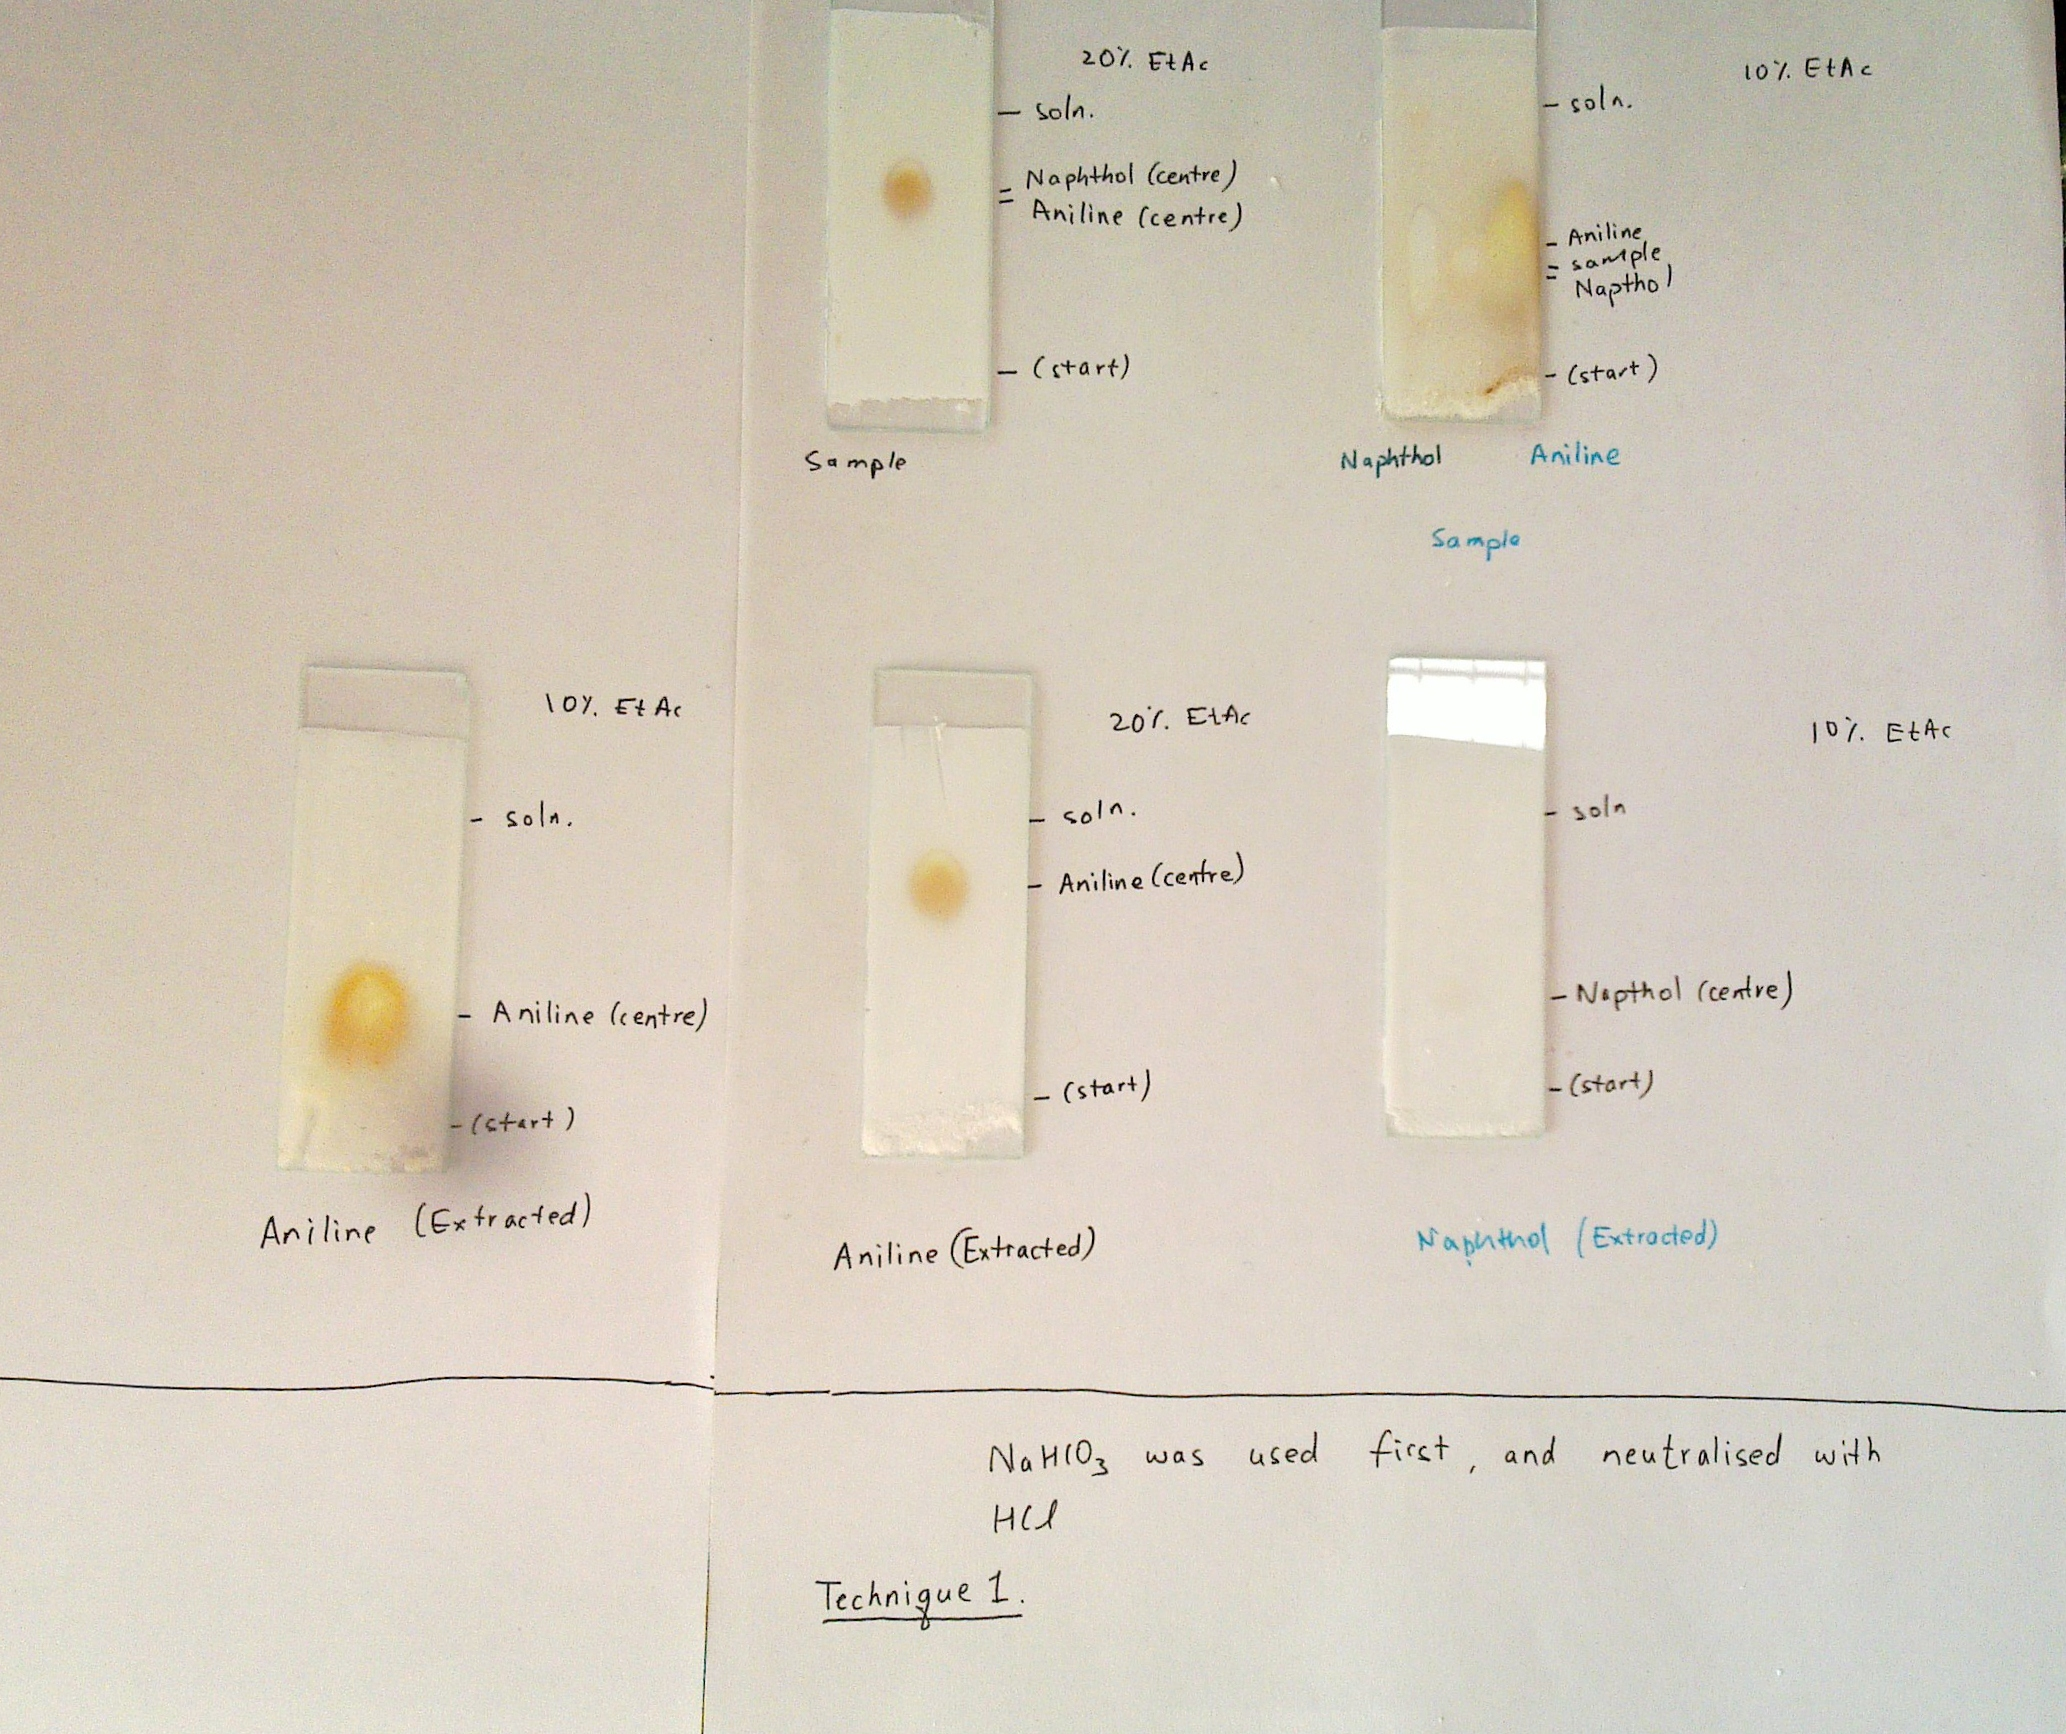
\includegraphics[width=1.5\linewidth]{gfx/e5_1}
	% 	\end{center}
	% \caption[TLCs Set 1]{\label{e5_1}}
	% \end{figure}

	% \begin{figure}[bth]
	% 	\begin{center}
	% 		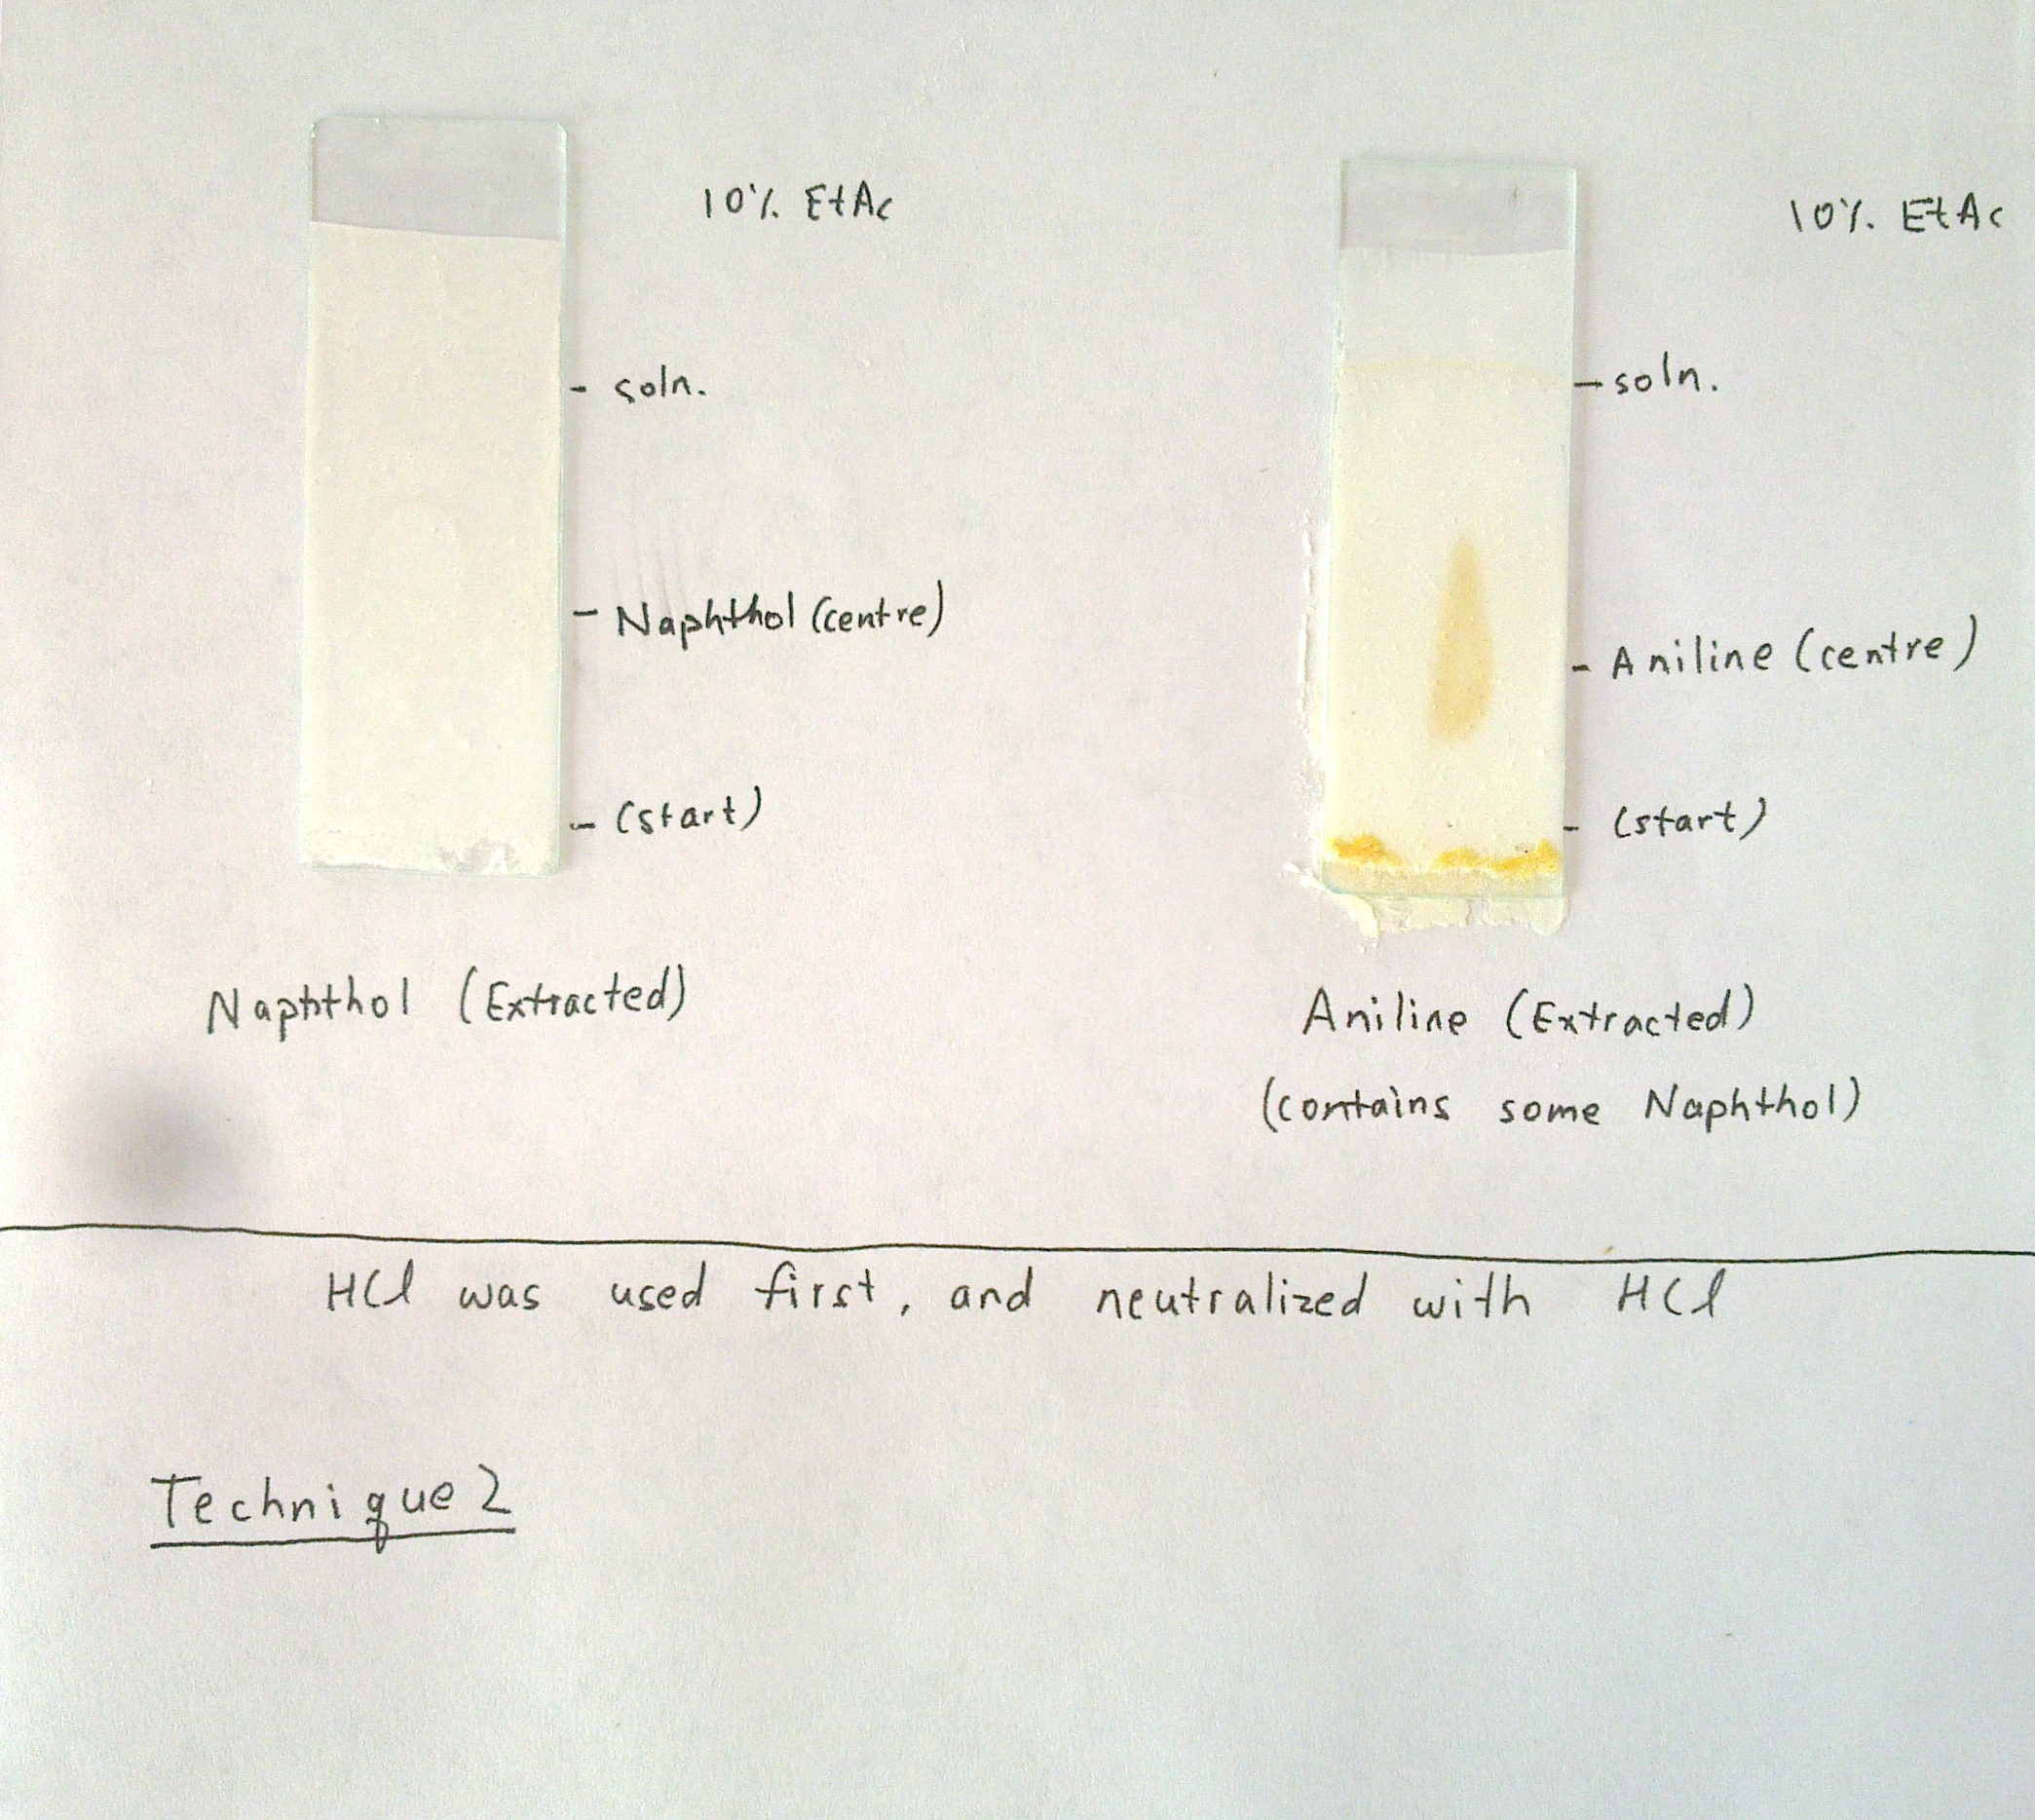
\includegraphics[width=1.0\linewidth]{gfx/e5_2}
	% 	\end{center}
	% \caption[TLCs Set 2]{\label{e5_2}}
	% \end{figure}